\subsection{Control of the car}\label{sprint2:car_control}
At the interview the stakeholders expressed that they needed to change how the car was controlled.
They wanted the car to reflect the current sound level of the speech recorded by the microphone.
This is expressed in requirement \ref{sprint2:tab1:req2} in \cref{sprint2:requirement_table_1}.

This has been implemented in the game by mapping the values recorded by the microphone to a range that corresponds to the height of the road.
This mapping is shown on \cref{mapping}.
The microphone records sounds and outputs values between 0 and some max value, shown as 1000 for simplicity.
When calibrating the microphone two values are defined, the minimum value reflecting background noise caught by the microphone, and the maximum value determined by the sound level of the player's shouting.
These two values are mapped to values between 0 and the height of the road, in the example 800.

The returned value is the position on the screen where the car needs to drive towards at the current sound level.

\begin{figure}
\centering
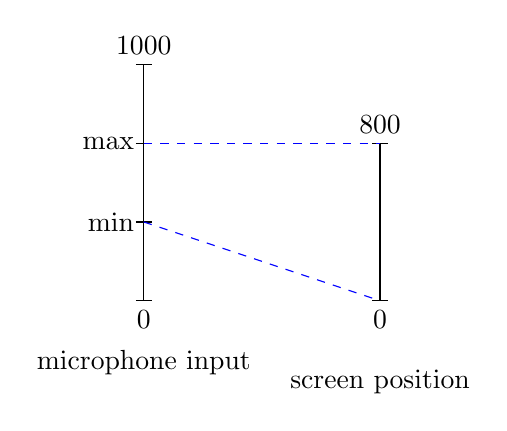
\begin{tikzpicture}
%vertical scales
\draw (0,0) -- (0,3); 
\draw (3,0) -- (3,2);

\node [below] at (0,-0.5){microphone input};
\node [below] at (3,-0.75){screen position};

%  endpoints with labels
\draw (-0.1,0) -- (0.1,0); 
\node [below] at (0,0){0};

\draw (-0.1,3) -- (0.1,3);
\node [above] at (0,3){1000};

\draw (2.9,0) -- (3.1,0); 
\node [below] at (3,0){0};

\draw (2.9,2) -- (3.1,2);
\node [above] at (3,2){800};

%min and max labels 
\draw (-0.1,1) -- (0.1,1);
\node [left] at (0,1){min};

\draw (-0.1,2) -- (0.1,2);
\node [left] at (0,2){max};

% mapping lines
\draw [dashed, blue](0,2) -- (3,2);
\draw [dashed, blue](0,1) -- (3,0);
\end{tikzpicture}
\caption{The mapping from microphone input to position on the screen}
\label{mapping}
\end{figure}
